
\chapter{\"Uberblick und Zielstellung}
Auf Basis eines XMOS-Mikrocontrollers mit angeschlossenem Kameramodul, haben wir
im Rahmen dieses Projekts einen Codec zur \"Ubertragung der Bilddaten entwickelt.
Hauptaugenmerk lag dabei darauf, die Komprimierung der Daten auf Streambasis
durchzuf\"uhren, also den Speicherbedarf aufgrund der Hardwarebesch\"rankungen 
weitestgehend zu minimieren.\\
Abbildung~\ref{fig:cam-stream} zeigt die Formatierung der Bilddaten, wie sie von
der Kamera erwartet werden. Die Flags NEWFRAME und NEWLINE werden mit einer
Breite von 32~Bit als 0xFFFFFFFF oder entsprechend 0xFEFEFEFE kodiert. Die
Implementierung der De- und Encoder sind jedoch von der Kodierung der
Kameradaten losgel\"ost. Um unabh\"angig von der Kamera-Hardware zu entwickeln,
existiert zus\"atzlich ein in XC geschriebener Testgenerator, der solch ein
Datenstream zur Verf\"ugung stellt.
%
\begin{figure}[htbp]
\begin{center}
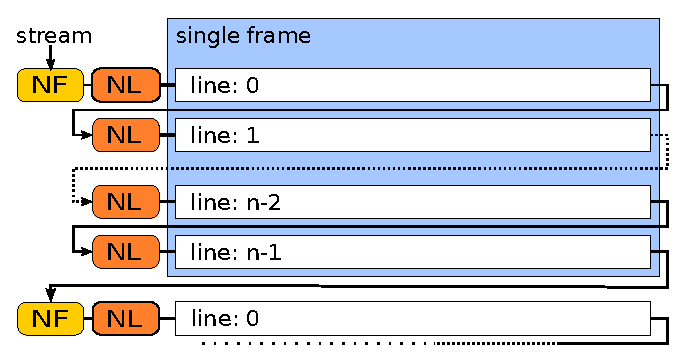
\includegraphics{img/cam-stream}
\end{center}
\caption{Formatierung des Kamera-Streams}
\label{fig:cam-stream}
\end{figure}

Um die Integrit\"at des Codecs zwischen Plattformen - z.B. XMOS-Transmitter 
und UNIX-Receiver - zu gew\"ahrleiten, haben wir die De- und Encoder
in reinem~C geschrieben. Somit konnten wir zus\"atzlich auf Verwendung Pointern
zur\"uckgreifen, was uns einigen redundanten Code ersparrt hat. Infolge dessen
mussten wir lediglich APIs f\"ur die jeweilige Plattform implementieren.
